\documentclass[11pt, a4paper, twocolumn]{article}
\usepackage{graphicx}
\graphicspath{ {images/} }
\usepackage{caption}
\usepackage{subcaption}
\usepackage{url}
\captionsetup[figure]{font=small}
\title{Song Feature Analysis}
\author{Jason Liu, Jordan Conragan, Kanak Kshirsagar}
\date{November 2021}

\begin{document}
\maketitle
\section{Abstract}
Genres are the mainstream way of musical classification, however, artists and producers of certain genres could have styles that vary greatly. The music produced could have significantly different musical features even while falling under the same umbrella for the genre. In this paper, we look to analyze whether it is possible to classify the genre of music tracks based on features found in a Spotify dataset. In order to solve this problem, we applied several methods including: the use of forward variable selection with logistic regression and SVM to produce an accuracy score of 45 percent, the use of decision tree classification to produce a result of 50 percent, and PCA with K-Means clustering to look at the distribution of tracks to features and genres. With this study, we were able to identify important features between genres. Due to the many overlapping features between genres, we conclude that logistic regression and decision tree classification failed to classify genres based on their features. 
\section{Introduction}	
Music can be seen as a medium to bring people together. However, when someone asks "What type of music do you like?", it could bring about unnecessary complications. Modern music even with the same genre can be vastly different in terms of musical features. Genre labels serve as very broad terms that classify the music of specific types, however, different artists of a specific genre might have vastly different styles. In this paper, we analyze the possibility of classifying music based on musical features.

The dataset that we will be using is a Spotify dataset that contains a total of 6 broad genres. These genres include alternative, blues, hip hop, indie alternative, metal, pop, and rock. The dataset contains a total of 22 columns. The following are the main features that we'll be interested in during our analysis. 
\begin{itemize}
\item Danceability: How suitable a track is for dancing. 
\item Energy: The precepted intensity of a track. 
\item Loudness: Overall decibels(dB)
\item Speechiness: Measures the presence of spoken words.
\item Acousticness: A confidence measure of whether or not a track is acoustic. 
\item Instrumentalness: Measures the lack of presence of vocals. 
\item Liveness: The likelihood that a track was performed live.
\item Valence: The conceptual musical positivity of a track. 
\item Tempo: The speed or pace of the track. 
\end{itemize}
\subsection{Preprocessing}
We clean the dataset by trimming features such as playlist, id, uri, track href, analysis url, and genres. For our methods listed below, we will using the subset of traits as listed above. Across this subset, we will be performing basic data exploration to visualize the data. This will act as a precursor in recognizing any potential patterns that may occur during the later phase of our analysis. The methods that we will be applying to the dataset include logistic regression, SVM, PCA, K-Means clustering, and decision trees. 
\subsection{Data Exploration}
We used boxplots in order to analyze the distribution of data for each of the features across the seven genres of music. By observing these boxplots, we made predictions about which features would be relevant for distuishing each genre. Here is a selection of those plots, as well as the predictions we made based on those plots before any analysis was performed.
\begin{figure}[htb!]
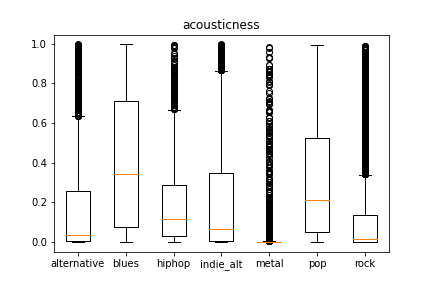
\includegraphics[scale=0.5]{acousticness}
\caption{Box Plot of Acousticness}
\end{figure}
The median and upper-quartile acoustics for blues are significantly higher than any other genre. This indicates that acousticness will be a good variable for distinguishing it from other genres. Furthermore, the median for acoustincess shows a wide range of variance, so this may end up being a good variable for several different genres.
\begin{figure}[htb!]
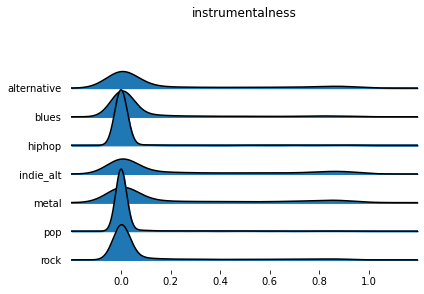
\includegraphics[scale=0.5]{instrumentalness}
\caption{Box Plot of Instrumentalness}
\end{figure}
The boxplot for instrumentalness is interesting because the median for all genres is relatively small, but the range and upper-quartile seem to vary widely. Due to its variability, instrumentalness could be another variable that is good for distinguishing several different genres.
\begin{figure}[htb!]
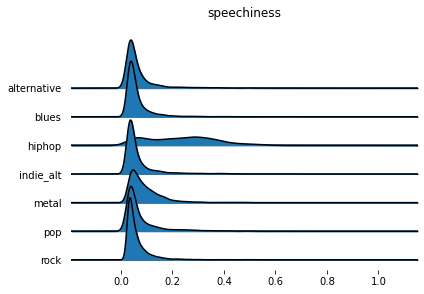
\includegraphics[scale=0.5]{speechiness}
\caption{Box Plot of Speechiness}
\end{figure}
The median and upper-quartile speechiness for hip hop is significantly higher than any other genre. This means that speechiness will most likely be an excellent variable for distinguishing hip hop songs. This makes sense logically because hip hop is heavily focused on lyrics and not instrumentals.
\subsubsection{Ridgeline Plots}
Ridgeline plots were another tool that we used during our data exploration. These plots helped to visualize the frequency of features across genres and allowed us to determine if there were any possible connections between features. 
\begin{figure}[htb!]
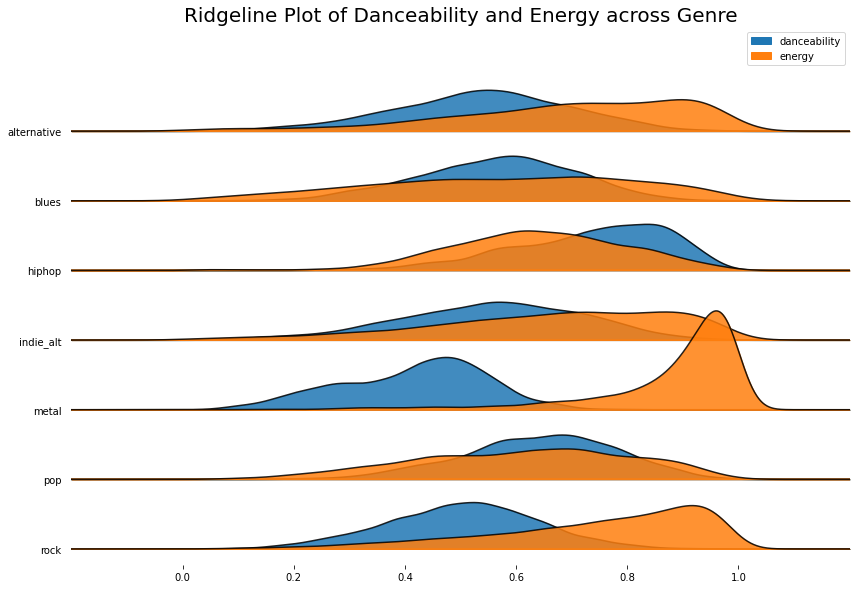
\includegraphics[scale=0.25]{dne}
\caption {Ridgeline Plot Comparing Danceability v. Energy}
\end{figure}
Figure 4 shows a ridgeline plot mapping danceability against energy across all genres. This allowed us to visualize the high danceability in hip hop as well as the higher energy in metal and rock. This shows that high energy does not directly correlate to high danceability. 
\begin{figure}[htb!]
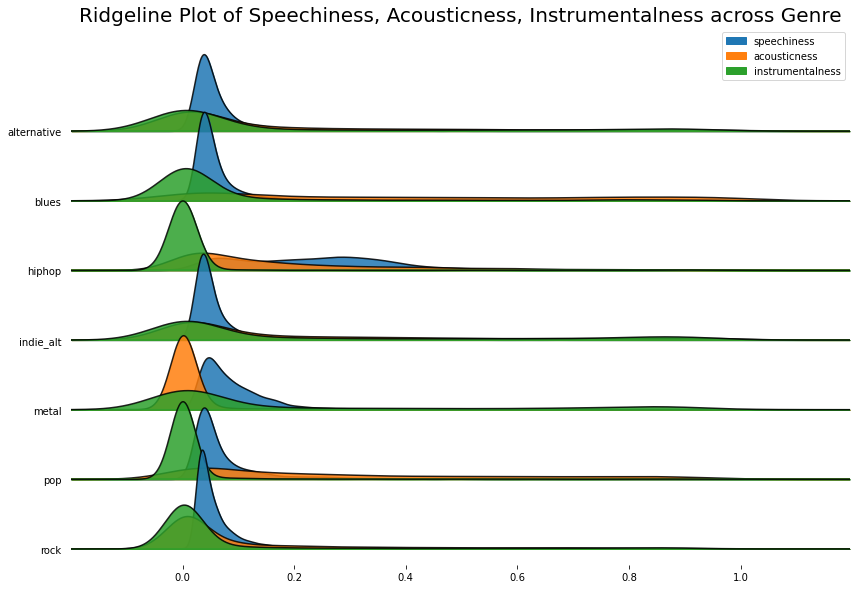
\includegraphics[scale=0.25]{sai}
\caption{Ridgeline plot comparing Speechiness, Acousticness, and Instrumentalness}
\end{figure}
Figure 5 shows the mapping of speechiness, acousticness, and instrumentalness across all the genres. This figure shows that hiphop has a significantly higher speechiness. It also shows that indie alt. and metal both have a higher distribution of instrumentalness compared to the other genres. These will be some of the relations we look forward to checking during our analysis. 
\subsection{Stats}

\begin{figure}[htb!]
\centerline{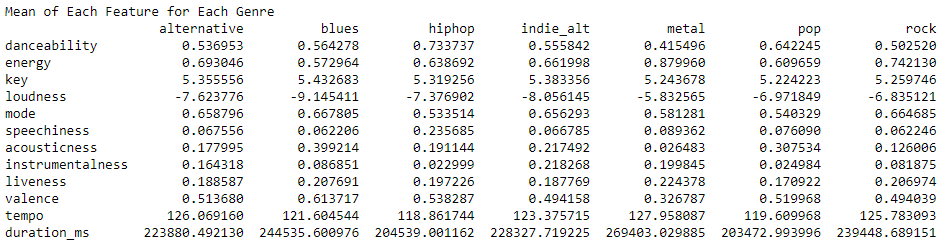
\includegraphics[scale=0.3]{Stats_Mean}}
\caption{Mean for each feature across all genres}
\end{figure}
\begin{figure}[htb!]
\centerline{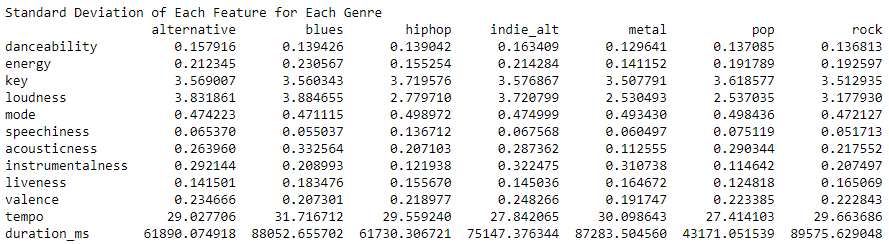
\includegraphics[scale=0.3]{Stats_SD}}
\caption{Standard Deviation for each feature across all genres}
\end{figure}
We were able to generate the corresponding mean and standard devaitions for features across genres, however, it was difficult to draw any meaningful conclusions at this stage of the analysis. Significant findings at this stage are that metal has a mean of 0.880 for energy, hip hop has a mean of 0.734 for danceability, and blues has a mean of 0.399 for instrumentalness. On average these genres were 1 standard deviation above the other genres for their respective features.
\section{Methods and Analysis}
\subsection{Logistic Regression}
One of the questions we wanted to solve was what variables are important for distinguishing songs from each genre? We answered this question using logistic regression.

There are a three main reasons why we chose to use logistic regression: it's fast, it's good at binary classification, and it's interpretable. We needed to build many logistic models for our analysis, and so it was convenient to have an algorithm that would run quickly. For our analysis, we needed a model that answers the question: "is a given song genre x, or is it any other genre?" Logistic regression is good at those kinds of problems. The last and most important factor is that logistic regression gives interpretable results. We could have used PCA or neural networks to identify important variables, but the results of both methods are difficult to interpert. We wanted to say "blues music is characterized by high acousticness", not "blues music is characterized by this principal component of eigenvalues." Another reason is that we tried to use the P values of the logistic model's coefficients, but that method gave us inconclusive results.

To identify the important variables for each genre, we measured how much each variable impacts the performance of the logistic model for that genre. We used forward variable selection (building a logistic model for each genre with 1 variable, then 2 variables, etc) to narrow down and rank the most influential variables. We measured model performance by comparing each model's AIC score. Since we're trying to understand the underlying patterns of our data, not build a classifier, we don't care about the model's predicted accuracy.

The models were trained using a '1 vs many' algorithm in which each genre will be independently measured against a collection of all other genres. In order to balance our model, during the training process we use the same amount of songs from the 1 genre vs the many genres. For example, while training the model for metal we used 3045 songs from the metal genre along with a random pool of 3045 songs from all the other genres.

We found the three most important variables for distinguishing genres. We chose three variables because it will give us a rounded understanding of each genre without having too many variables to analyze. Figure 8 shows a table containing those variables.
\begin{figure}[htb!]
\centerline{\includegraphics[scale=0.85]{Log_Reg_Table}}
\caption{Primary Features of Genres}
\end{figure}
This table reveals some interesting patterns. Instrumentalness, acousticness, and especially speechiness are influential variables for many different genres. This matches some of our initial predictions about our data. Based on the boxplots we created, we identified instrumentalness and acousticness as possibly being important (and as expected, it was an important variable for distinguishing the blues). We also thought that hip hop would be primarily defined by its speechiness. This is because hip hop relies heavily on its lyrics and because its average speechiness was significantly higher than any other genre (see Figure 6 for a breakdown on the mean values of each feature for each genre).

We were surpsied that speechiness is such an important variable for many genres other than hip hop. Likewise for acousticness. We also expected that metal, which had a significantly higher average energy than the other genres, would be primarily defined by that feature. However, the only genre that is is influenced by its energy is hip hop.

Our logistic regression analysis was successful at determining which variables are significant for distinguishing each genre. However, our analysis does have two major restrictions.

First, we cannot determine how well each variable defines a particular genre. Instrumentalness may be the best way to distinguish a pop song from other genres of music, but it cannot be used to identify 10 percent of pop songs (and every other variable is worse) nor can it alone be used to identify a pop song with 70 percent accuracy? We're not testing the accuracy of our logistic model, and logistic regression doesn't have a good metric to tell us how well it works. The AIC score for logistic regression is good for comparing the accuracy of two models, but it is poor at determining the overall performance of our model. R\textsuperscript{2}, which works well for linear regression, doesn't work well for logistic regression. However, there is a solution to this. We can build a genre classifier using the variables that we determined were important, which is what we do in the next section.

Secondly, this analysis doesn't tell us how each variable distinguishes a genre. We know that one important variable for distignuishing metal songs is the length of each song, however, we don't know whether metal songs are longer than most other songs, shorter than most other songs, or fit somwhere in the middle for the range of durations. We can remedy this by combining this analysis with the statistics we calculated earlier. For example, we can see that the average song duration for metal songs is longer than the average duration for most other genres. This means that an important characterisic of metal music is that its songs are longer than other genres.
\subsection{SVM}
In a previous analysis, we identified the most important variables that distinguish a particular genre from the rest. The next part of our analysis is building a classifier that can identify the genre of a song. In this section, we use a mutli-class support vector machine to build that classifier.

One strength of SVMs is that they are flexible. An SVM with a linear kernel acts works well on linear data, but an SVM with an exponential kernel is good for classifying exponential data. The library we're using, libsvm, supports a wide variety of kernels and SVM implementations. This allowed us to tune the parameters of the SVM to work best with our dataset.

Our song dataset is imbalanced towards certain genres (particularly rock and roll), so to combat this, we trained the SVM on the same number of songs frome each genre. The least-represented genre in our is the blues, which only has 2050 songs. We rounded that number down to 2000 songs from each genre. We wanted to avoid overfitting our data, so we only used variables that were relevant for distinguishing genres. We used the instrumentalness, acousticness, speechiness, energy, duration ms, valence, danceability, loudness from each song to build our training dataset. We then used k-fold cross validation to train and evaluate our SVM model.
\begin{figure}[htb!]
\centerline{\includegraphics[scale=0.85]{svm}}
\caption{SVM Model Parameters}
\end{figure}
Figure 9 shows the parameters and hyperparameters that we used to create the optimal model. We found these through trial and error. Despite our efforts to create a good model, the k-fold cross validation of our model is only 45 percent. There are two possible reasons for this.

SVMs are not appropriate for analyzing our dataset. The variables in the dataset are not appropraite for creating an effective classifier. In a later analysis, we create another song genre classifier using decision trees. Its accuracy was not significantly higher than the cross-validation accuracy we got using an SVM. This indicates that the second conslusion is true, and that our dataset is insufficient to create an accurate classifier.
\subsection{Decision Tree}
The second analysis method used for classification was decision trees. Decision tree classification was used to understand how the decision rules use different feature subsets to classify genres. 
\begin{figure}[htb!]
\centerline{\includegraphics[scale=0.9]{DecisionTreeText}}
\caption{Textual Representation of Decision Tree Results}
\end{figure}
For our decision trees, we used the training and testing approach. We split our data into a training set with 70 percent of the data (18726 rows),  and a testing set with 30 percent of the data (8026 rows). The first iterations of the tree produced results that were difficult to visualize due to the size of the tree. In order to combat this, we pruned the tree by modifying the minimal-cost complexity parameter, \texttt{ccp\char`_alpha}, to control the size of the tree and avoid over-fitting. By modifying the \texttt{ccp\char`_alpha} input for the decision tree, the smallest effective alpha nodes were pruned first. Through various iterations of trial and error modifying \texttt{ccp\char`_alpha}, we were able to obtain a maximum accuracy score of 50 percent on the decision tree. 

The rules from the decision tree show some interesting features used to classify the genres. The main observations of the decision tree results are as followed: Danceability (as observed from Logistic Regression) and acousticness are used for rock, instrumentalness along with tempo is used to determine metal, valence and liveness are used to classify hiphop. The accuracy score of 50 percent indicates that decision trees were not a good fit for the classification of song features to genre. This is similar to the results produced through logistic regression and SVM. 

\subsection{PCA and K-Means Clustering}
Since we were not able to achieve acceptible accuracy scores using features to genre classification, the last methods that we used to analyze our dataset were Principal Component Analysis or PCA and K-Means clustering. One of the reasons we used PCA with K-Means clustering was to see how the music would be clustered based on features only without regard to genre. By doing this we can see the distribution of features to genre per cluster. The reason PCA was chosen was because our feature set had a high number of features and PCA would handle the dimensionality reduction aspect. After using PCA to handle the dimensionality reduction we could use K-Means clustering to classify the results. 
For PCA and K-Means clustering, we used a test set of 700 samples, 100 tracks from each of the 7 genres. Furthermore we drom the irrelevant features. The features that were included in this analysis include: danceability, energy, speechiness, acousticness, instrumentalness, liveness, valence, and tempo. Before we subject this subset of data to PCA and K-Means we also apply sklearn's standardscaler in order to factor in the different scales that tempo uses. 
\subsubsection{PCA}
PCA is a dimensionality reduction technique that can help to reduce the number of components provided from a dataset while minimalizing data loss \cite{pca}. After scaling our dataset we applied PCA in order to determine the explained variance ratio across the number of components by using sklearn's PCA package. The cumulative explained variance is the sum of variances from all of the individual principal components\cite{cev}. Figure 11 shows a mapping of cumulative explained variable for each component. The dotted line across 0.8 which indicates a cumulative explained variance of at least 80 percent which is the standard acceptible amount. Figure 11 indicates that for this subset of data we would need 5 components to maintain an acceptible level of explained variance. This is interesting because from the mean average determined in Figure 6 two of the features which did not show much variance throughout genres were liveness and tempo. 
\begin{figure}[htb!]
\centerline{\includegraphics[scale=0.285]{PCA Variance}}
\caption{Cumulative Explained Variance over Number of Components}
\end{figure} 

After determining how many components to use in our PCA we can calculate how many clusters to use in our K-Means clustering by checking the inertia between clusters. For this, we calculate the inertia for each of the clusters ranging from 0 to 20. Figure 12 shows a chart plotting the WCSS (Within-Cluster Sum of Squares), the sum of squared distance between each point and centroid of cluster. The higher the number of clusters the lower the WCSS value, after a certain drop-off (Elbow), increasing the number of clusters fail to provide significant differences. This allows us to choose the optimal amount of clusters for producing significant results. One of the problems encountered with our analysis was that there was not a clear elbow as indicated by figure 12, however, it appears that the curve has a reduction in steepness at around 6 to 7 clusters. We tested our following K-Means clustering with 7 clusters.
\begin{figure}[htb!]
\centerline{\includegraphics[scale=0.285]{Elbow}}
\caption{WCSS Across Clusters}
\end{figure}
\subsubsection{K-Means Clustering}
After figuring out the number of components and optimal number of clusters to use, 5 and 7, respectively we were able to create clusters based scores created by our PCA model after training with the subset. 
\begin{figure}[htb!]
\centerline{\includegraphics[scale=0.285]{K700}}
\caption{Scatter Plot of K-Means Cluster}
\end{figure}
\begin{figure}[htb!]
\centerline{\includegraphics[scale=0.285]{fRadar}}
\caption{Mean of Features across Clusters}
\end{figure}
Figures 13 and 14 show that we were able to create clusters based on musical features without relations to the provided genre. The following is a brief summary of features significant to each cluster: 
\begin{itemize}
\item Cluster 0: Moderate Energy
\item Cluster 1: Valence and Danceability
\item Cluster 2: Energy and Tempo
\item Cluster 3: Energy and Liveness
\item Cluster 4: Speechiness and Danceability
\item Cluster 5: Instrumentalness
\item Cluster 6: Accousticness 
\end{itemize} 
One sample that we closely exampled was cluster 5. Cluster 5 had a distribution of 48 tracks which accounts for 6.8 percent of the tracks tested. Cluster 5 had a distribution of genres as follows: 16 Metal, 13 Alternative, 10 Indie Alternative, 5 Blues, 4 Rock. The following bar graph in figure 15 shows the distribution of instrumentalness for each of the tracks in the cluster, we can see that the instrumentalness values are much higher than the average across 700 samples which is indicated by the red horizontal line. We can conclude that clustering based on features alone create clusters with significant differences based only on their musical features. Through this experiment we were able to create a playlist of songs featured in cluster 5, link provided in the references section \cite{spotify}.
\begin{figure}[htb!]
\centerline{\includegraphics[scale=0.285]{C5Inst}}
\caption{Cluster 5 Distribution of Instrumentalness Across Track}
\end{figure}
 Through K-Means clustering we can see that the basis of failure for our previous analysis is true because it is very hard to distinguish genres of music solely based on features. There are many features that overlap per musical genre so it makes sense that the accuracy ratings for our classification did not exceed 50 percent. Clustering music based on its features may be a better way to organize music rather than by genre. 
\section{Conclusion}
Through our analysis of the Spotify dataset, we were able to identify the features that were significant to each genre. By using logistic regression we were able to figure out the three main defining features of a genre, and through decision tree classification we were able to confirm similar results. Although we were able to glean features of significance in relation to genre, we were not able to fully classify the music based solely on their features. Through logistic regression and SVM we were able to achieve a maximum accuracy score of 45 percent and through our decision tree classification an accuracy score of 50 percent. Combining these results with the results of our PCA and K-Means clustering we can confirm that although the clustering of music based on feature is possible classification is very difficult. 
\begin{thebibliography}{5}
\bibitem{pca}
Ian T. J. and Jorge C. (2016) \emph{Principal component anlysis: a review and recent developments}, Philosophical Transcations of the Royal Society A: Mathematical, Physical and Engineering Sciences \url {https://doi.org/10.1098/rsta.2015.0202}
\bibitem{spotify}
Jason Liu (2021) \url{https://open.spotify.com/playlist/1yJgzfX3D3K7875gGp2n76?si=eab8e5c1d7294c0c&nd=1}, Accessed: Dec 9, 202
\bibitem{cev}
Roman Cheplyaka (2017) \emph{Exaplined variance in PCA} \url{https://ro-che.info/articles/2017-12-11-pca-explained-variance}, Accessed: Dec. 9, 2021
\end{thebibliography}
\end{document}